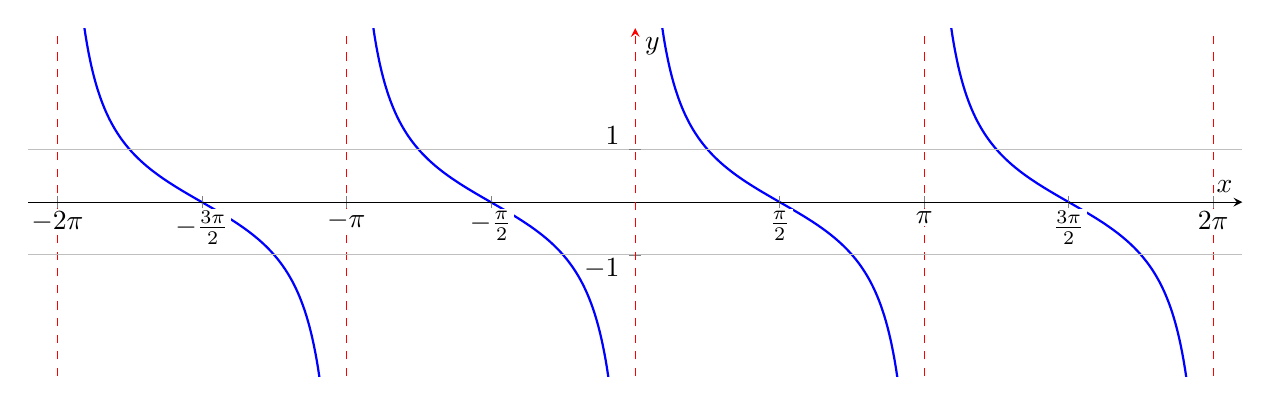
\begin{tikzpicture}
    \begin{axis}
        [
            width = 17cm,
            height = 6cm,
            axis lines = middle,
            axis on top = true,
            y axis line style = {red, dashed},
            xlabel = {$x$},
            ylabel = {$y$},
            xmin = -6.6,
            xmax = 6.6,
            ymin = -3.3,
            ymax = 3.3,
            xtick = {-2*pi, -3*pi/2, -pi, -pi/2, 0, pi/2, pi, 3*pi/2, 2*pi},
            xticklabels = {
                    $-2\pi$,
                    $-\frac{3\pi}{2}$,
                    $-\pi$,
                    $-\frac{\pi}{2}$,
                    $0$,
                    $\frac{\pi}{2}$,
                    $\pi$,
                    $\frac{3\pi}{2}$,
                    $2\pi$
                },
            xticklabel style = {fill = white, inner sep = 1pt},
            ytick = {-1, 0, 1},
            yticklabel style = {yshift = {\tick*5pt}},
            grid = major,
            xmajorgrids = false,
            samples = 201,
        ]

        % Tiệm cận đứng: x = k*pi; x = 0 trùng với trục Oy nét đứt.
        \pgfplotsinvokeforeach{-2, -1, 1, 2}
        {
            \draw[red, dashed]
                (axis cs:{#1*pi}, -3.3) -- (axis cs:{#1*pi}, 3.3);
        }

        % Vẽ riêng từng nhánh để không nối qua các tiệm cận.
        \addplot[blue, thick, domain = -2*pi+0.01:-pi-0.01]
            {cos(deg(x))/sin(deg(x))};
        \addplot[blue, thick, domain = -pi+0.01:-0.01]
            {cos(deg(x))/sin(deg(x))};
        \addplot[blue, thick, domain = 0.01:pi-0.01]
            {cos(deg(x))/sin(deg(x))};
        \addplot[blue, thick, domain = pi+0.01:2*pi-0.01]
            {cos(deg(x))/sin(deg(x))};
    \end{axis}
\end{tikzpicture}
